%%%%%%%%%%%%%%%%%%%%%%%%%%%%%%%%%%%%%%%%%%%%%%%%%%%%%%%%%%%%%%%
%
% Welcome to Overleaf --- just edit your LaTeX on the left,
% and we'll compile it for you on the right. If you open the
% 'Share' menu, you can invite other users to edit at the same
% time. See www.overleaf.com/learn for more info. Enjoy!
%
%%%%%%%%%%%%%%%%%%%%%%%%%%%%%%%%%%%%%%%%%%%%%%%%%%%%%%%%%%%%%%%
\documentclass{beamer}

%Russian-specific packages
%--------------------------------------
\usepackage[T2A]{fontenc}
\usepackage[utf8]{inputenc}
\usepackage[russian]{babel}
%--------------------------------------
 
%Hyphenation rules
%--------------------------------------
\usepackage{hyphenat}
\hyphenation{ма-те-ма-ти-ка вос-ста-нав-ли-вать}
%--------------------------------------

%Paragraph spacing%
\setlength{\parskip}{1em}
%---------------------


%Information to be included in the title page:
\title{Статически оптимальное дерево отрезков}
\author{Артем Комендантян, 4 курс МФТИ, кафедра анализа данных \\
\small{Научный руководитель: Михаил Тихомиров, к.ф.-м.н.}
}
\date{2021}

\addtobeamertemplate{navigation symbols}{}{%
    \usebeamerfont{footline}%
    \usebeamercolor[fg]{footline}%
    \hspace{1em}%
    \insertframenumber/\inserttotalframenumber
}

\begin{document}

\frame{\titlepage}

\begin{frame}
\frametitle{Определения}
Пусть дан массив из $n$ элементов

\textbf{Дерево отрезков} - это двоичное дерево, в котором есть

\begin{itemize}
\item $n$ листьев, соответствующих отрезкам единичной длины
\item Вершины с двумя сыновьями. Правый сын соответствует отрезку, следующему сразу за отрезком левого сына. Вершина соответствует объединению отрезков сыновей
\end{itemize}
Корень дерева соответствует всему массиву (отрезку $[1; n]$)

\end{frame}

\begin{frame}
\frametitle{Определения}

\textbf{Запрос сверху} на отрезке $[L, R]$ начинается в корне.

Если сейчас рассматривается вершина, отрезок которой не лежит полностью в отрезке $[L, R]$, то запрос рекурсивно вызывается от тех сыновей, отрезки которых пересекаются с $[L, R]$. Иначе рекурсивных вызовов от сыновей не происходит.

В обоих случаях вершина считается посещенной и в ней выполняются какие-то действия, специфичные для запроса.

\end{frame}

\begin{frame}
\frametitle{Пример}

\begin{columns}
\column{0.5\textwidth}
Дерево отрезков на пяти элементах

Запрос на отрезке $[2; 4]$

Посещено пять выделенных вершин

\column{0.5\textwidth}
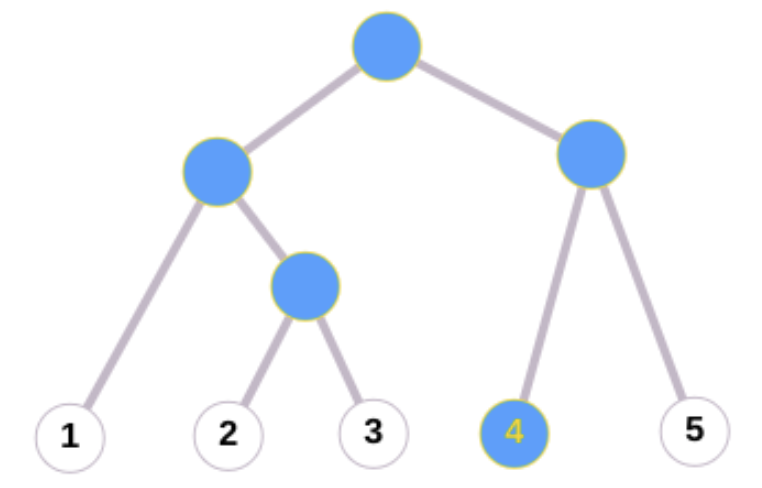
\includegraphics[scale=0.22]{segtree_example.png}
\end{columns}

\end{frame}

\begin{frame}
\frametitle{Постановка задачи}

\textbf{Дано:} Распределение вероятностей на запросах-отрезках с границами из $[1; n]$

\textbf{Необходимо:} построить дерево отрезков, для которого минимально среднее количество посещенных вершин при запросах сверху.

Интересует как точное решение за как можно более лучшую асимптотику, так и приближенное за сложность нахождения $O(n + S)$ или $O(n + S \log S)$, где $S$ - количество отрезков с ненулевой вероятностью.

\end{frame}

\begin{frame}
\frametitle{Мотивация}

\begin{itemize}
\item Дерево отрезков - мощная структура, позволяющая эффективно решать множество задач. Примеры: наименьший общий предок двух вершин в дереве, площадь объединения прямоугольников со сторонами, параллельными осям координат
\item Потенциальное ускорение в реальных задачах
\item Аналогичная задача для деревьев поиска хорошо изучена

\end{itemize}

\end{frame}

\begin{frame}
\frametitle{Статически оптимальное двоичное дерево поиска}

\textbf{Дано:} множество из $n$ упорядоченных элементов и $2n + 1$ вероятностей, что запрос будет равен элементу из множества, либо находиться между двух соседних элементов

\textbf{Необходимо:} построить двоичное дерево поиска, для которого минимально среднее количество посещенных вершин при запросах

\end{frame}

\begin{frame}
\frametitle{Обзор решений}

\begin{itemize}
\item \textbf{Точное решение:} динамическое программирование за $O(n^3)$ времени и $O(n^2)$ памяти, оптимизируется до $O(n^2)$ времени [1].
\item Обобщение задач, к которым применима данная оптимизация [3]
\item Точное решение за $O(n \log n)$ времени для случая, когда запросы поступают только между элементов [4]
\item \textbf{Приближенное решение:} жадное решение за O(n), хуже оптимального не более чем в константу раз, где константа примерно равна 2.283... [2]  \\ Идея решения - выбирать такой корень, чтобы максимально уравнять сумму вероятностей в левом и правом поддереве, затем перейти к двум меньшим подзадачам

\end{itemize}

\end{frame}

\begin{frame}
\frametitle{Вернемся к нашей задаче}

\end{frame}

\begin{frame}
\frametitle{Точное решение}

\begin{itemize}
\item Нам даны веса-вероятности запросов
\item $dp_{L, R}$ - суммарный вес оптимального дерева отрезков, построенного на точках с $L$ по $R$
\item Для каждого запроса оставляем пересечение с $[L, R]$
\item Либо не рассматриваем, если не пересекается
\end{itemize}

\end{frame}

\begin{frame}
\frametitle{Точное решение}

\begin{itemize}
\item Для отрезка $[L, R]$ к весу дерева отрезков прибавляется сумма весов запросов, которые пересекаются с $[L, R]$
\item Если сыновьям корня соответствуют отрезки $[L, m]$ и $[m + 1, R]$, надо учесть вес дерева отрезков на $[L, m]$ и на $[m + 1, R]$
\item Запросы целиком содержащие $[L, R]$ не нужно учитывать в сыновьях
\end{itemize}


\end{frame}

\begin{frame}
\frametitle{Точное решение}

\begin{itemize}
\item Отсюда dp_{L, R} = cost_{L, R} + \min \limits_{L \le m < R} {dp_{L, m} + dp_{m + 1, R}}$
\item Восстановление дерева по оптимальным $m$
\item Функция стоимости $cost_{L, R}$ ищется перебором за $O(n^2S)$
\item Можно выразить её слагаемые рекурсивно и находить за $O(n^2)$
\item Итоговое решение за $O(n^3)$ времени и $O(n^2)$ памяти
\end{itemize}

\end{frame}


\begin{frame}
\frametitle{Идеи для более оптимального решения}
В [3] было показана возможность оптимизации до $O(n^2)$, если
\begin{itemize}
\item $\forall a \le b \le c \le d:\ cost_{a, d} \ge cost_{b, c}$ (монотонность)
 \item $\forall a \le b \le c \le d:\ cost_{a, c} + cost_{b, d} \le cost_{a, d} + cost_{b, c}$ (quadrangle неравенство)
\end{itemize}

В нашей задаче
\begin{itemize}
\item Первое неравенство верно
\item Второе верно с противоположным знаком
\end{itemize}

\end{frame}



\begin{frame}
\frametitle{Приближенное решение}

\begin{itemize}
\item Сейчас: Число посещенных вершин запроса $[L, R]$
\item Меняем на сумму максимальных глубин запросов $[1, R]$ и $[L, n]$
\item Веса запросов оставляем те же
\item Было доказано, что старое и новое значение запросов отличаются не более чем в два раза
\item Оптимальное решение для новой задачи не более чем в четыре раза хуже оптимального для старого

\end{itemize}

\end{frame}

\begin{frame}
\frametitle{Частный случай запроса}

\begin{columns}
\column{0.5\textwidth}
Посещенные вершины $[L, R]$

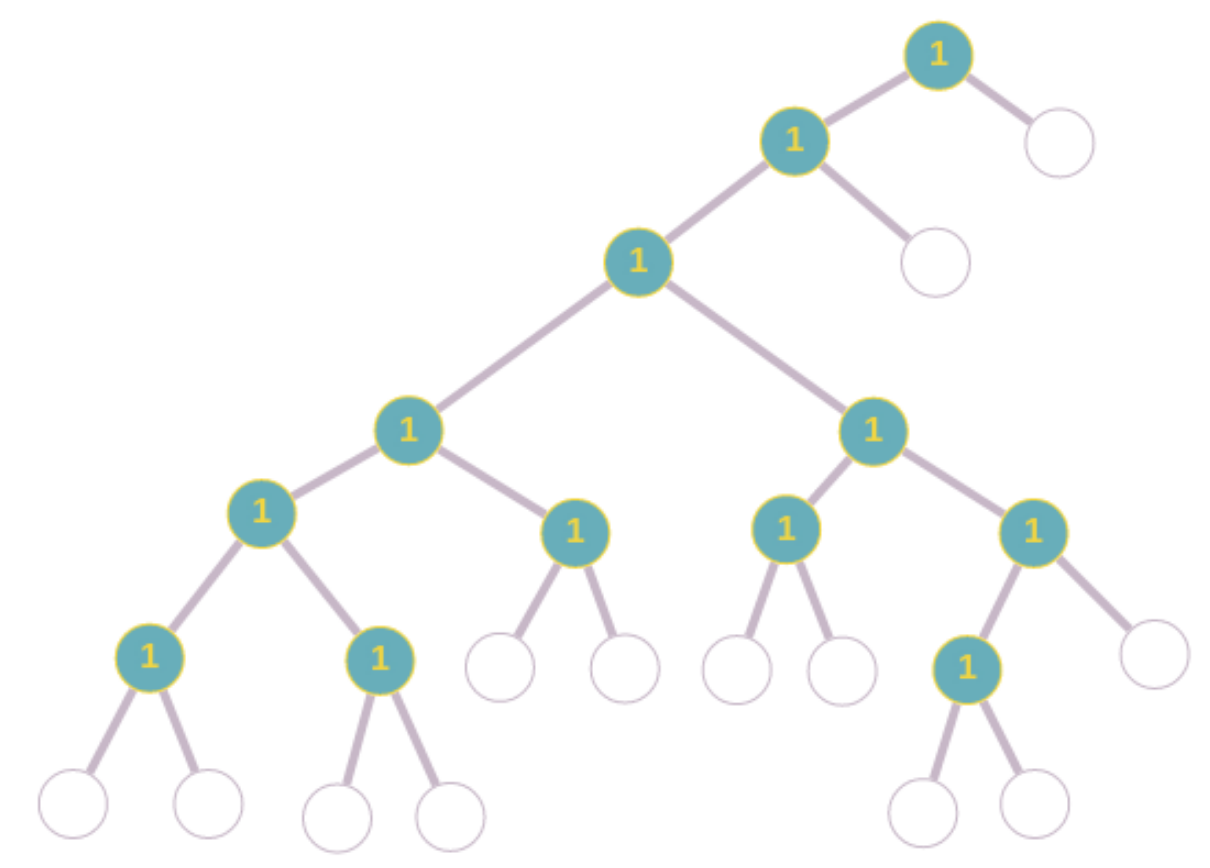
\includegraphics[scale=0.13]{segtree_old.png}

\column{0.5\textwidth}
Сумма глубин $[1, R]$ и $[L, n]$

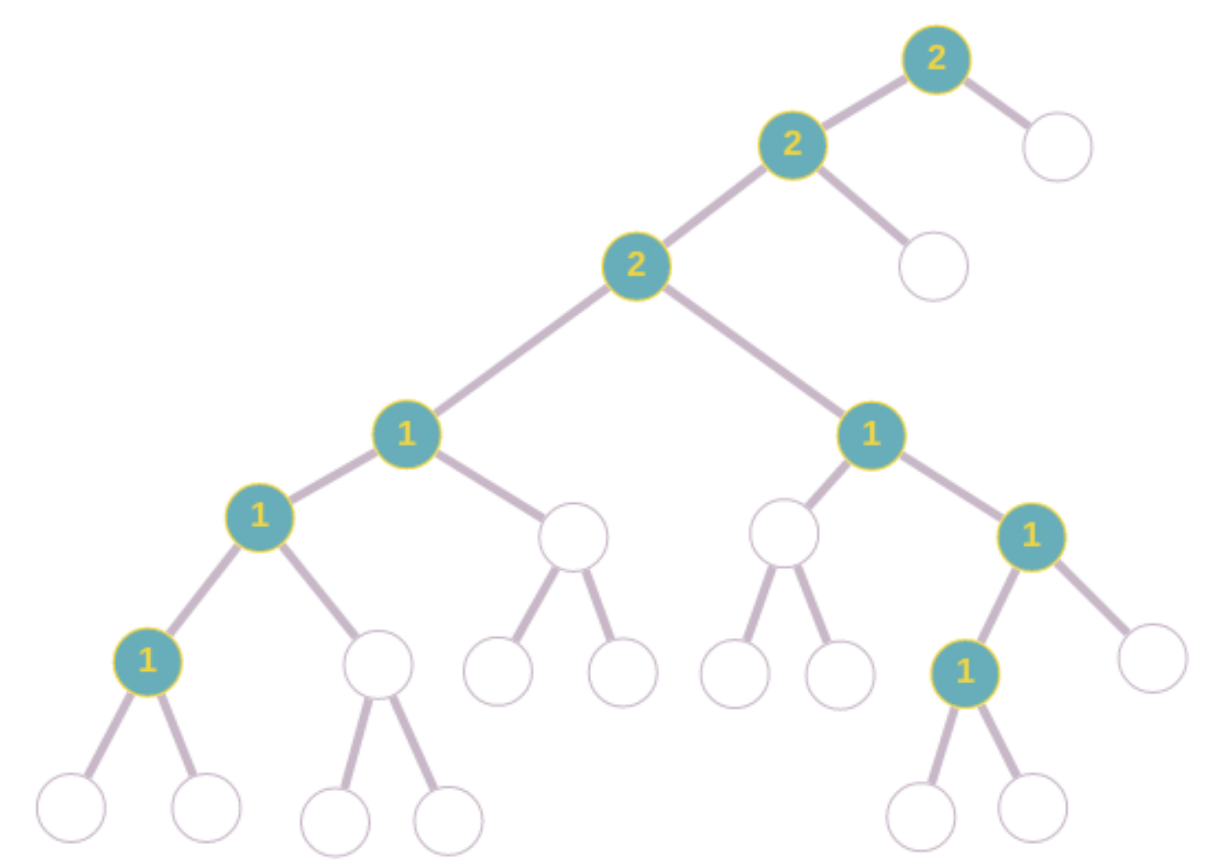
\includegraphics[scale=0.13]{segtree_depth.png}
\end{columns}

\small{(для каждой вершины отмечено, сколько она раз учтётся в ответе)}

\begin{itemize}
\item До какой-то глубины вклад в ответ в два раза больше справа
\item После этого не более чем в два раза больше слева
\item Общий случай разбирается похожим образом
\end{itemize}

\end{frame}

\begin{frame}
\frametitle{Приближенное решение}

\begin{itemize}
\item $lw_i$ - сумма весов запросов $[i, n]$
\item $rw_i$ - сумма весов запросов $[1, i]$
\item $w_i = rw_i + lw_{i + 1}$
\item $dp_{L, R}$ - стоимость оптимального дерева отрезков с новыми запросами, построенного на точках с $L$ по $R$ 
\item $dp_{L, R} = \sum \limits_{L}^{R - 1} w_i + \min \limits_{L \le m < R} {dp_{L, m} + dp_{m + 1, R}}$
\item Эквивалентно задаче об оптимальном дереве поиска с вероятностями элементов пропорциональными $w_1,\dots,w_{n-1}$
\end{itemize}

\end{frame}


\begin{frame}
\frametitle{Приближенное решение}

Из сведения, [1] и [2] получаем два приближенных решения:

\begin{itemize}
\item За $O(n^2 + S)$ времени и не более чем в четыре раза хуже оптимального
\item За $O(n + S)$ времени и не более чем в $\approx 4 \cdot 2.283 = 9.132$ раз хуже оптимального
\end{itemize}

\end{frame}


\begin{frame}
\frametitle{Приближенное решение на практике}

\begin{itemize}
\item Случайные тесты с $n \le 100$ и $S$ от $1$ до $n^2$
\item Решение за $O(n^2 + S)$ не более чем в $\approx 1.42$ раз хуже оптимального
\item Решение за $O(n + S)$ не более чем в $\approx 2.3$ раз хуже оптимального
\item Значения сравнимы с константой для приближенного нахождения дерева поиска
\item И уже могут иметь не только теоретический интерес
\end{itemize}

\end{frame}


\begin{frame}
\frametitle{Спасибо за внимание!}

\end{frame}

\begin{frame}
\frametitle{Список литературы}
\begin{enumerate}
\item  Knuth, Donald E. (1971), "Optimum binary search trees", Acta Informatica.

\item Mehlhorn, Kurt (1975), "Nearly optimal binary search trees", Acta Informatica.

\item F. Frances Yao (1980), "Efficient Dynamic Programming Using Quadrangle Inequalities".

\item Garsia, Adriano M.; Wachs, Michelle L. (1977), "A new algorithm for minimum cost binary trees", SIAM Journal on Computing.

\end{enumerate}

\end{frame}

\end{document}